\documentclass[conference]{IEEEtran}
\usepackage[utf8]{inputenc}
\usepackage{amsmath,amssymb,graphicx,booktabs}

\usepackage[hidelinks,unicode,pdftitle={SLERP versus LERP for Merging Qwen2.5-0.5B Base and Instruct: A Paired Comparison on ARC, HellaSwag, and WinoGrande},pdfauthor={Dheiver Francisco Santos},pdfkeywords={model merging, SLERP, linear interpolation, weight space, Qwen2.5, paired bootstrap},pdfsubject={Preprint, Figshare, doi:10.6084/m9.figshare.35013982}]{hyperref}
\begin{document}

\title{SLERP versus LERP for Merging Qwen2.5-0.5B Base and Instruct: A Paired Comparison on ARC, HellaSwag, and WinoGrande}

\author{\IEEEauthorblockN{Dheiver Francisco Santos, PhD}
\IEEEauthorblockA{Independent Researcher\\
Maceió, Alagoas, Brazil\\
ORCID: https://orcid.org/0000-0002-8599-9436\\
Preprint, Figshare, 2026, \href{https://doi.org/10.6084/m9.figshare.35013982}{doi:10.6084/m9.figshare.35013982}, CC BY 4.0}}

\maketitle

\begin{abstract}
Spherical linear interpolation (SLERP) is an alternative to linear interpolation (LERP) for merging fine-tuned language models. We merge Qwen2.5-0.5B and its Instruct sibling at four coefficients with both operators and score macro accuracy on 3{,}967 held-out items from four benchmarks. The pre-registered hypothesis was that SLERP does not differ from LERP. Paired SLERP$-$LERP test differences range from $-0.10$ to $+0.35$ percentage points (pp), and every 95\% bootstrap interval contains zero. No difference was detected (no equivalence test). The 95\% interval for the exploratory mean difference is $[-0.09,+0.39]$ pp. The test used bfloat16 weights, whose rounding is about ten times larger than the relative SLERP--LERP gap, and about 90\% of merged elements are identical after the cast. On validation in fp32, the difference is $0.00$ and $-0.17$ pp at $t=0.4$ and $0.6$ (bf16: $+0.25$ and $+0.42$): the size of precision noise, with the sign reversed at $t=0.6$. The primary comparison, a validation-chosen SLERP merge against the best original model, is not distinguishable ($+0.40$ pp, $p=0.262$). One model pair.
\end{abstract}

\begin{IEEEkeywords}
model merging, SLERP, linear interpolation, weight space, Qwen2.5, paired bootstrap
\end{IEEEkeywords}

\section{Introduction}
Merging the weights of two models that share an ancestor is a training-free way to obtain a third model. For a base model and its instruction-tuned descendant, the simplest recipe is linear interpolation of the parameters, $(1-t)\theta_b+t\theta_i$. A frequently used alternative is spherical linear interpolation, which interpolates along the arc between the two weight vectors instead of the chord. SLERP is implemented in open merging toolkits \cite{goddard2024mergekit} and is often used on the premise that it preserves the geometry of the weights better than the chord; this premise is our motivation for the test, not a claim we verify. In the literature we reviewed, we found no controlled, paired comparison against LERP on a held-out benchmark.

This paper asks one narrow question: for the pair Qwen2.5-0.5B and Qwen2.5-0.5B-Instruct \cite{qwen25}, does SLERP give a different accuracy than LERP at the same coefficient $t$, and does choosing the coefficient by validation make either operator beat the best original model? The hypothesis was written before any merge was run: SLERP does not differ from LERP, because the two checkpoints are close. We report the outcome. A null result of this kind is only as informative as the interval width allows.

Contributions: (i) a paired item-level comparison of SLERP and LERP at four coefficients with bootstrap intervals; (ii) measured weight-space angles and SLERP--LERP distances, which are consistent with the two operators coinciding for this pair; (iii) an analytic small-angle argument for why they coincide whenever the angle is small, kept apart from the measurements; and (iv) a validation-selected merge compared with the best original model, reported as not distinguishable.

\section{Related Work}
\textbf{SLERP and its origin.} SLERP was introduced for animating rotations expressed as unit quaternions \cite{shoemake1985slerp}, where the interpolant must stay on the sphere. Its use on neural weights borrows the formula but not the constraint: weight tensors are not unit vectors, and no result known to us shows that the sphere is the right manifold for them. The open-source toolkit MergeKit exposes SLERP next to linear averaging, task arithmetic, TIES and DARE, and thousands of community models have been merged with it \cite{goddard2024mergekit}. The gap we address is the absence of a paired accuracy comparison between the two interpolation geometries at matched coefficients.

\textbf{Geometry of weights and connectivity.} Whether interpolation between two weight vectors is useful depends on the loss along the path. Linear mode connectivity shows that networks that share early training remain connected by a low-loss line \cite{frankle2020lmc}, and permutation symmetries can make independently trained networks connectable after alignment \cite{ainsworth2022rebasin}. Fine-tuned descendants of one pre-trained model often appear to lie in a single low-error basin. This is the regime of weight averaging and model soups \cite{wortsman2022soups} and of interpolation between zero-shot and fine-tuned weights \cite{wortsman2022wiseft}. It is also the regime of averaging with Fisher information or regression-based weights \cite{matena2021fisher,jin2022dataless}. All of these operate near the chord, and we did not find a paired chord-versus-arc comparison.

\textbf{Merging methods and surveys.} Task arithmetic adds scaled differences between fine-tuned and pre-trained weights \cite{ilharco2022editing}; TIES and DARE remove redundant or conflicting parameter updates \cite{yadav2023ties,yu2023dare}; evolutionary and adaptive search tunes recipes or coefficients \cite{akiba2024evolutionary}; a survey catalogues these operators \cite{yang2024survey}, and another covers weight-averaging and mode-connectivity-based fusion \cite{li2023fusion}. A study of merging at scale reports how base-model strength and size affect merging outcomes \cite{yadav2024matters}. These works vary the operator class; we hold the pair fixed and vary only the interpolation geometry, which isolates the question.

\textbf{Author's related work.} The author's technical notes cover neighboring topics in language-model training: model merging for capability composition \cite{santos2026modelmergingfo}, knowledge distillation and self-distillation \cite{santos2026knowledgedisti}, parameter-efficient fine-tuning (LoRA, QLoRA, DoRA) \cite{santos2026parametereffic}, mixture-of-experts training and sparse upcycling \cite{santos2026mixtureofexper}, curriculum learning and data-efficient pretraining \cite{santos2026curriculumlear}, synthetic data generation and self-improvement \cite{santos2026syntheticdatag}, direct preference optimization \cite{santos2026directpreferen}, and RLAIF and Constitutional AI \cite{santos2026rlaifandconsti}. This paper instead reports a controlled held-out measurement. In a different domain, the author's JEPA preprint \cite{santos2026collapseresist} uses a similar controlled-comparison style (identical budgets, several seeds, confidence intervals).

\section{Method}
Let $a=\theta_b$ and $b=\theta_i$ denote one parameter tensor of the base and the instruct model, flattened to a vector. With coefficient $t\in[0,1]$ ($t=0$ is the base, $t=1$ is the instruct model), the two operators act tensor by tensor:
\begin{align}
\theta^{\mathrm{LERP}}_t &= (1-t)\,a+t\,b, \label{eq:lerp}\\
\Omega &= \arccos\frac{\langle a,b\rangle}{\lVert a\rVert\,\lVert b\rVert}, \label{eq:angle}\\
\theta^{\mathrm{SLERP}}_t &= \frac{\sin((1-t)\Omega)}{\sin\Omega}\,a+\frac{\sin(t\Omega)}{\sin\Omega}\,b. \label{eq:slerp}
\end{align}
Our implementation computes $\Omega$ per tensor on the flattened tensor, and falls back to LERP for a tensor when either norm is below $10^{-8}$ or $\Omega<10^{-4}$. Merging is done in fp32 on the CPU; the result is copied into a bfloat16 model.

\subsection*{Equations and their meaning}
Eq.~(\ref{eq:lerp}) moves along the straight line between the two weight vectors; the point at $t=0.4$ is 40\% of the way from the base to the instruct model. Eq.~(\ref{eq:angle}) is the angle $\Omega$ between the two tensors seen as vectors: $\Omega=0$ means they point in the same direction. Eq.~(\ref{eq:slerp}) moves along the arc between the two directions; its two coefficients are not $1-t$ and $t$ but sines of fractions of that angle, so the arc coefficients differ from the line coefficients by an amount that depends on $\Omega$.

\textbf{Analytic argument (not measured).} For small $\Omega$, $\sin(s\Omega)/\sin\Omega = s\,[1+(1-s^2)\Omega^2/6]+O(\Omega^4)$. Applying this with $s=1-t$ and $s=t$ gives
\begin{equation}
\theta^{\mathrm{SLERP}}_t-\theta^{\mathrm{LERP}}_t=\frac{\Omega^2}{6}\,t(1-t)\,\big[(2-t)\,a+(1+t)\,b\big]+O(\Omega^4). \label{eq:gap}
\end{equation}
Since $(2-t)+(1+t)=3$, the norm of the bracket is at most $3\max(\lVert a\rVert,\lVert b\rVert)$, so for nearly parallel tensors the relative gap is of order $\tfrac{\Omega^2}{2}\,t(1-t)\le\Omega^2/8$. As the angle goes to zero, the arc and the chord coincide, and SLERP$\to$LERP at rate $\Omega^2$. If the two norms are equal, $\lVert b-a\rVert/\lVert a\rVert=2\sin(\Omega/2)\approx\Omega$, so the relative norm of the task vector $\lVert\theta_i-\theta_b\rVert/\lVert\theta_b\rVert$ is of the same order as $\Omega$. For this pair that ratio is $0.0418$ (Section~\ref{sec:geometry}), but $0.0418$ is a ratio of norms, not the angle. The per-tensor median angle is $0.050$ rad and the element-weighted mean angle is $0.085$ rad (\texttt{results/extras\_art02\_03.json}). At $t=0.4$ the estimate $\Omega^2 t(1-t)/2$ is $3.0\times10^{-4}$ with the median angle and $8.7\times10^{-4}$ with the weighted angle, so it is an order-of-magnitude estimate, not a bound. The measured global gap ($2.9\times10^{-4}$ to $4.4\times10^{-4}$) is of the order of the estimate. It slightly exceeds the value from $\Omega=0.0418$ ($\approx2\times10^{-4}$ at $t=0.5$) because $0.0418$ is not the angle. Only the worst tensor ($\Omega=0.11$) reaches about $1.5\times10^{-3}$. The norms of base and instruct tensors are not exactly equal, and the link to accuracy (a tiny weight change gives a tiny accuracy change) is an assumption, not a theorem.

\section{Experimental Protocol}
\textbf{Models.} Qwen2.5-0.5B (revision \texttt{060db64}) and Qwen2.5-0.5B-Instruct (revision \texttt{7ae5576}), both Apache-2.0 \cite{qwen25}; full hashes are in \texttt{MANIFEST.json}. The merged weights are evaluated in bfloat16 with PyTorch on Apple Silicon (MPS).

\textbf{Data and splits.} Multiple-choice log-likelihood scoring in the style of the lm-evaluation-harness \cite{gao2021harness}: ARC-Easy and ARC-Challenge \cite{clark2018arc} and HellaSwag \cite{zellers2019hellaswag} (all three with accuracy normalized by answer length in characters, \texttt{acc\_norm}) and WinoGrande \cite{sakaguchi2019winogrande} (partial scoring, no normalization). The primary metric is the macro mean of the four accuracies. Splits are disjoint (seed 0): a validation set of 300 items per task (299 for ARC-Challenge; 1{,}199 in total) and a test set of 1{,}000 items per task (967 for WinoGrande; 3{,}967 in total). No selection uses test items; every grid point was also scored on test, as declared below.

\textbf{Selection.} Grid $t\in\{0.2,0.4,0.6,0.8\}$ for both operators, fixed in the pre-registration before any merge was run. The coefficient is chosen by the highest validation macro accuracy among the four SLERP merges; the endpoints $t=0$ and $t=1$ are the original models. The best original model is the one with the higher validation accuracy (base: $0.4953$; instruct: $0.4853$). Test accuracy of every grid point is reported to draw the curves, but no choice uses it.

\textbf{Baselines.} (a) The best original model chosen on validation (the base); (b) the instruct model; (c) LERP at the same $t$, evaluated at the same four coefficients and thus with the same selection budget as SLERP.

\textbf{Statistics.} Bootstrap over items with tasks equally weighted: 3{,}000 resamples for paired differences, 2{,}000 for a single accuracy. Differences are paired by item against the comparator; $p$ is two-sided from the bootstrap distribution (B=3,000: the smallest nonzero two-sided $p$ is 2/3,000). The pre-registration (\texttt{experiments/PREREG.md}) fixed 5,000 bootstrap resamples; the analysis used 2,000 for a single accuracy and 3,000 for paired differences. The pre-registered success rule was a paired 95\% CI above zero. Six primary comparisons across Articles 1--6 are corrected to a Bonferroni threshold of $0.05/6=0.0083$, which was added after the pre-registration; no comparison in this paper has a nominal $p<0.05$, so none requires the correction. The primary comparison is the SLERP merge chosen on validation against the best original model (the base). The SLERP$-$LERP differences at each $t$ are secondary, and the four-coefficient mean is an exploratory aggregate (the same resampled items are shared across coefficients). Merges are deterministic, so there is no seed variance to estimate; uncertainty is over items only.

\section{Results}
\subsection{Weight geometry}\label{sec:geometry}
Over the 290 parameter tensors of the Qwen2.5-0.5B state dictionary, the angle between base and instruct tensors is small: median $\Omega=0.050$ rad ($2.9^\circ$), 95th percentile $0.089$, maximum $0.110$ rad ($6.3^\circ$). The relative norm of the task vector $\lVert\theta_i-\theta_b\rVert/\lVert\theta_b\rVert$ over all tensors is $0.0418$. The measured relative $L_2$ distance between SLERP and LERP weights, over all tensors, is $2.9\times10^{-4}$ ($t=0.2$), $4.4\times10^{-4}$ ($t=0.4$), $4.4\times10^{-4}$ ($t=0.6$) and $2.9\times10^{-4}$ ($t=0.8$); the largest value in any single tensor is $1.5\times10^{-3}$ (at $t=0.4$ and $0.6$), which agrees with the estimate $\Omega^2 t(1-t)/2$ at the maximum angle. The relative gap (about $4\times10^{-4}$) is an order of magnitude below bfloat16 unit roundoff ($2^{-8}\approx3.9\times10^{-3}$). We measured the effect after casting SLERP and LERP weights to bf16 (\texttt{results/slerp\_bf16\_check.txt}): $0.8998$ ($t=0.4$) and $0.8991$ ($t=0.6$) of the elements are identical, and the relative $L_2$ distance is $8.8\times10^{-4}$ at both coefficients.

\subsection{SLERP versus LERP}
Table~\ref{tab:main} gives the paired differences on the test set. All four intervals contain zero, the smallest nominal $p$ is $0.158$, and the largest difference in absolute value is $0.35$ pp. The mean over the four coefficients is $+0.14$ pp (95\% CI $[-0.09,+0.39]$, $p=0.228$). The 95\% interval for the mean difference is $[-0.09,+0.39]$ pp. Across the four coefficients, the widest interval bounds exclude SLERP advantages above $+0.83$ pp and disadvantages below $-0.52$ pp. This is not a formal equivalence test with a pre-set margin. The validation differences in bf16 are $+0.08$, $+0.25$, $+0.42$ and $-0.33$ pp at $t=0.2,\dots,0.8$. We re-scored validation in fp32 at two coefficients (\texttt{results/slerp\_bf16\_check.txt}). At $t=0.4$, LERP and SLERP both score $0.4945$ (difference $0.00$ pp; bf16: $0.4953$ and $0.4978$, $+0.25$ pp). At $t=0.6$, LERP scores $0.4953$ and SLERP $0.4936$ ($-0.17$ pp; bf16: $0.4853$ and $0.4895$, $+0.42$ pp). The bf16 differences are therefore of the size of precision noise, and the sign reverses at $t=0.6$ when the weights are kept in fp32. These two points are validation only, with 1{,}199 items and no interval; the test set was not re-scored in fp32.

\begin{table*}[!t]
\caption{SLERP versus LERP on Qwen2.5-0.5B base$\leftrightarrow$instruct. Macro accuracy on validation ($n=1199$) and test ($n=3967$); the last two columns are the paired test difference with 95\% bootstrap CI and two-sided $p$. Original models: base val $0.4953$ / test $0.5025$; instruct val $0.4853$ / test $0.5064$.}
\label{tab:main}
\centering\small
\begin{tabular}{lcccccc}
\toprule
$t$ & Val SLERP & Val LERP & Test SLERP & Test LERP & SLERP$-$LERP (pp) [95\% CI] & $p$\\
\midrule
0.2 & 0.4953 & 0.4945 & 0.5007 & 0.4983 & $+0.24$ [$-0.23$, $+0.71$] & 0.318\\
0.4 & 0.4978 & 0.4953 & 0.5064 & 0.5029 & $+0.35$ [$-0.15$, $+0.83$] & 0.158\\
0.6 & 0.4895 & 0.4853 & 0.5094 & 0.5087 & $+0.07$ [$-0.41$, $+0.61$] & 0.778\\
0.8 & 0.4920 & 0.4953 & 0.5064 & 0.5074 & $-0.10$ [$-0.52$, $+0.32$] & 0.654\\
\midrule
Mean of four & --- & --- & --- & --- & $+0.14$ [$-0.09$, $+0.39$] & 0.228\\
\bottomrule
\end{tabular}
\end{table*}

\begin{figure}[!t]
\centering
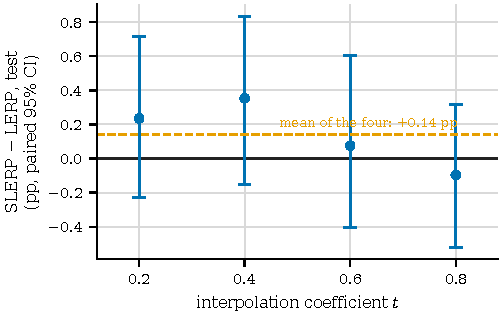
\includegraphics[width=\columnwidth]{figs/fig02_slerp_vs_lerp.pdf}
\caption{Paired test difference SLERP$-$LERP (pp) at each coefficient $t$, with 95\% bootstrap CI as error bars. The dashed line is the mean over the four coefficients. Every interval contains zero.}
\label{fig:fig02}
\end{figure}

\subsection{Validation-selected coefficient}
The validation set selects SLERP at $t^\ast=0.4$ (validation macro $0.4978$, the best of the four SLERP points). On the test set it scores $0.5064$ against $0.5025$ for the best original model chosen on validation (the base): $+0.40$ pp (95\% CI $[-0.29,+1.09]$, $p=0.262$). Against the instruct model the difference is $0.00$ pp (95\% CI $[-0.84,+0.85]$). The corresponding LERP merge at $t=0.4$ differs from the base by $+0.04$ pp (95\% CI $[-0.67,+0.76]$). The pre-registered success criterion (lower end of the interval above zero) is not met by either operator. No difference between the selected merge and the original models was detected, and the choice of operator does not change that (no equivalence margin tested). The relevant magnitude is the width of the interval, $\pm0.7$ pp, not the sign of the point estimate.

\textbf{What these results do not show.} They do not show that SLERP and LERP are equivalent for other model pairs, larger angles (for example models fine-tuned from different bases or after long continued pre-training), other benchmarks, generation quality, or other coefficients. Nor do they show that the weight-space argument causes the tie. The argument predicts a tiny weight difference and the accuracy difference is small, but we did not intervene on the angle, for instance with a synthetic pair of larger angle. Item-level noise also limits resolution: the paired intervals have half-widths of about $0.5$ pp, so smaller effects cannot be detected with 3{,}967 items.

\section{Discussion and Limitations}
For this pair, using the arc instead of the chord changes neither the weights in a practically meaningful way (relative gap below $1.5\times10^{-3}$ in every tensor) nor the measured accuracy beyond the noise. The practical reading is conditional. When a base model and its fine-tuned descendant have a small relative task-vector norm (here $0.0418$), the simpler LERP is sufficient, and the choice should be revisited for larger angles. Eq.~(\ref{eq:gap}) states the dependence explicitly, but we have measured it for this pair only.

Threats to validity. (i) A single 0.5B model pair, one benchmark family of multiple-choice log-likelihood tasks, one hardware setup. (ii) The test split is slightly easier than the validation split (about $0.50$ against about $0.495$ for the originals), so we compare gains rather than levels. (iii) Public benchmarks may be contaminated in the models; this affects both operators equally but cannot be measured here. (iv) Merges are deterministic, so seed variance is absent, and the item bootstrap does not capture variation in the choice of the four-point grid. (v) Selecting among four SLERP points on 1{,}199 validation items is an instance of adaptive reuse \cite{dwork2015reusable}, and the maximum of noisy scores is biased upward. The validation gap of $t^\ast$ over the base ($+0.25$ pp) is of the same order as the test gain, and neither is separable from noise. (vi) Per-tensor flattening is one of several SLERP definitions (per-layer and per-row variants exist), and we tested only this one. (vii) The aggregate over four coefficients was computed after the pre-registration and is exploratory. (viii) The test was run with bfloat16 weights, and this confounds the operator comparison: the relative SLERP--LERP gap ($\approx4\times10^{-4}$) is an order of magnitude below bf16 rounding ($\approx4\times10^{-3}$), and about $90\%$ of merged elements are identical after the cast. The bf16 differences (up to $+0.35$ pp on test) are of the size of this rounding. Validation in fp32 was measured at two coefficients only ($t=0.4$ and $0.6$; difference $0.00$ and $-0.17$ pp against $+0.25$ and $+0.42$ pp in bf16); fp32 was not measured on test. An earlier fp32 re-evaluation of validation accuracy for the LERP path covered $t=0$, $0.7$ and $1$ (fp32: $0.4886$, $0.4920$, $0.4845$; shifts of $0.67$, $0.41$ and $0.08$~pp), and $t=0.7$ is not a grid point of this paper (\texttt{results/fp32\_check\_qwen.txt}). Exact accuracy levels are specific to bfloat16. Accuracy comparisons use paired intervals in the spirit of recommendations for error bars on evaluations \cite{miller2024errorbars}, with the bootstrap of Efron \cite{efron1979bootstrap}.

\section{Conclusion}
The pre-registered expectation that SLERP does not differ from LERP for Qwen2.5-0.5B base and instruct was not rejected: no difference was detected, and no equivalence margin was tested. The four paired differences are at most $0.35$ pp and all intervals contain zero. The 95\% interval for the exploratory mean difference is $[-0.09,+0.39]$ pp. The primary comparison, a validation-selected SLERP merge against the best original model, gives $+0.40$ pp (95\% CI $[-0.29,+1.09]$), not distinguishable from zero. In fp32 on validation the SLERP$-$LERP difference is $0.00$ and $-0.17$ pp (bf16: $+0.25$ and $+0.42$), so the bf16 gaps are of the size of precision noise. The measured angle between the checkpoints (median $0.050$ rad) and the relative SLERP--LERP weight gap (at most $1.5\times10^{-3}$) are of the order given by the small-angle estimate, which remains analytic. The next measurement is a model pair with a much larger angle, where Eq.~(\ref{eq:gap}) no longer predicts a negligible gap.

\section*{Data and Code Availability}
\sloppy
Repository: git tag \texttt{preprints-v1} (the commit that contains this manuscript and all scripts and caches). Per-item results for every evaluation are cached in \texttt{cache/} (\texttt{q\_slerp\_*}, \texttt{q\_lerp\_*}). Single command: \texttt{./run\_everything.sh}; the weight-geometry and aggregate statistics come from \texttt{experiments/an\_art02\_03.py}, written to \texttt{results/extras\_art02\_03.\{json,txt\}}, and the task-vector norms from \texttt{experiments/an\_taskvec.py}. Libraries: Python 3.9.6, PyTorch 2.8.0, transformers 4.57.6, numpy 1.26.4, datasets 4.5.0. Model revisions (Hub commits): Qwen2.5-0.5B \texttt{060db6499f32faf8\allowbreak b98477b0a26969ef7d8b9987}; Qwen2.5-0.5B-Instruct \texttt{7ae557604adf67be\allowbreak 50417f59c2c2f167def9a775}. Pre-registration: \texttt{experiments/PREREG.md}. Raw summary: \texttt{results/summary\_art02.txt}.

\section*{Acknowledgments}
No external funding.

\begin{thebibliography}{99}
\bibitem{shoemake1985slerp} K. Shoemake, ``Animating rotation with quaternion curves,'' in \emph{Proc. ACM SIGGRAPH}, 1985. doi:10.1145/325165.325242.
\bibitem{goddard2024mergekit} C. Goddard, S. Siriwardhana, M. Ehghaghi \emph{et al.}, ``Arcee's MergeKit: A toolkit for merging large language models,'' in \emph{Proc. EMNLP (Industry Track)}, 2024. arXiv:2403.13257.
\bibitem{ilharco2022editing} G. Ilharco, M. T. Ribeiro, M. Wortsman \emph{et al.}, ``Editing models with task arithmetic,'' in \emph{Proc. ICLR}, 2023. arXiv:2212.04089.
\bibitem{wortsman2022soups} M. Wortsman, G. Ilharco, S. Y. Gadre \emph{et al.}, ``Model soups: Averaging weights of multiple fine-tuned models improves accuracy without increasing inference time,'' in \emph{Proc. ICML}, 2022. arXiv:2203.05482.
\bibitem{wortsman2022wiseft} M. Wortsman, G. Ilharco, J. W. Kim \emph{et al.}, ``Robust fine-tuning of zero-shot models,'' in \emph{Proc. CVPR}, 2022. arXiv:2109.01903.
\bibitem{frankle2020lmc} J. Frankle, G. K. Dziugaite, D. M. Roy \emph{et al.}, ``Linear mode connectivity and the lottery ticket hypothesis,'' in \emph{Proc. ICML}, 2020. arXiv:1912.05671.
\bibitem{ainsworth2022rebasin} S. K. Ainsworth, J. Hayase, and S. Srinivasa, ``Git Re-Basin: Merging models modulo permutation symmetries,'' in \emph{Proc. ICLR}, 2023. arXiv:2209.04836.
\bibitem{matena2021fisher} M. Matena and C. Raffel, ``Merging models with Fisher-weighted averaging,'' in \emph{Proc. NeurIPS}, 2022. arXiv:2111.09832.
\bibitem{jin2022dataless} X. Jin, X. Ren, D. Preotiuc-Pietro \emph{et al.}, ``Dataless knowledge fusion by merging weights of language models,'' in \emph{Proc. ICLR}, 2023. arXiv:2212.09849.
\bibitem{yadav2023ties} P. Yadav, D. Tam, L. Choshen \emph{et al.}, ``TIES-Merging: Resolving interference when merging models,'' in \emph{Proc. NeurIPS}, 2023. arXiv:2306.01708.
\bibitem{yu2023dare} L. Yu, B. Yu, H. Yu \emph{et al.}, ``Language models are Super Mario: Absorbing abilities from homologous models as a free lunch,'' in \emph{Proc. ICML}, 2024. arXiv:2311.03099.
\bibitem{akiba2024evolutionary} T. Akiba, M. Shing, Y. Tang \emph{et al.}, ``Evolutionary optimization of model merging recipes,'' \emph{Nat.\ Mach.\ Intell.}, 2025, arXiv:2403.13187.
\bibitem{yang2024survey} E. Yang, L. Shen, G. Guo \emph{et al.}, ``Model merging in LLMs, MLLMs, and beyond: Methods, theories, applications and opportunities,'' arXiv:2408.07666, 2024.
\bibitem{li2023fusion} W. Li, Y. Peng, M. Zhang \emph{et al.}, ``Deep model fusion: A survey,'' arXiv:2309.15698, 2023.
\bibitem{yadav2024matters} P. Yadav, T. Vu, J. Lai \emph{et al.}, ``What matters for model merging at scale?'' arXiv:2410.03617, 2024.
\bibitem{qwen25} Qwen Team, A. Yang \emph{et al.}, ``Qwen2.5 technical report,'' arXiv:2412.15115, 2024.
\bibitem{clark2018arc} P. Clark, I. Cowhey, O. Etzioni \emph{et al.}, ``Think you have solved question answering? Try ARC, the AI2 reasoning challenge,'' arXiv:1803.05457, 2018.
\bibitem{zellers2019hellaswag} R. Zellers, A. Holtzman, Y. Bisk \emph{et al.}, ``HellaSwag: Can a machine really finish your sentence?'' in \emph{Proc. ACL}, 2019. arXiv:1905.07830.
\bibitem{sakaguchi2019winogrande} K. Sakaguchi, R. Le Bras, C. Bhagavatula, and Y. Choi, ``WinoGrande: An adversarial Winograd schema challenge at scale,'' in \emph{Proc. AAAI}, 2020. arXiv:1907.10641.
\bibitem{gao2021harness} L. Gao \emph{et al.}, ``EleutherAI/lm-evaluation-harness,'' Zenodo, doi:10.5281/zenodo.10256836.
\bibitem{efron1979bootstrap} B. Efron, ``Bootstrap methods: Another look at the jackknife,'' \emph{Ann. Statist.}, vol. 7, no. 1, 1979. doi:10.1214/aos/1176344552.
\bibitem{miller2024errorbars} E. Miller, ``Adding error bars to evals: A statistical approach to language model evaluations,'' arXiv:2411.00640, 2024.
\bibitem{dwork2015reusable} C. Dwork, V. Feldman, M. Hardt \emph{et al.}, ``Preserving statistical validity in adaptive data analysis,'' arXiv:1411.2664, 2014.
\bibitem{santos2026modelmergingfo} D. F. Santos, ``Model Merging for Capability Composition: A Technical Note,'' Zenodo, 2026, doi:10.5281/zenodo.21610555.
\bibitem{santos2026collapseresist} D. F. Santos, ``Collapse-Resistant Joint-Embedding Predictive Architectures: A Controlled Comparison of SIGReg, VICReg, and EMA,'' Zenodo, v2, 2026, doi:10.5281/zenodo.24223364.
\bibitem{santos2026knowledgedisti} D. F. Santos, ``Knowledge Distillation and Self-Distillation for Language Models,'' Zenodo, 2026, doi:10.5281/zenodo.21610100.
\bibitem{santos2026parametereffic} D. F. Santos, ``Parameter-Efficient Fine-Tuning: LoRA, QLoRA, and DoRA,'' Zenodo, 2026, doi:10.5281/zenodo.21610033.
\bibitem{santos2026mixtureofexper} D. F. Santos, ``Mixture-of-Experts Training and Sparse Upcycling,'' Zenodo, 2026, doi:10.5281/zenodo.21610062.
\bibitem{santos2026curriculumlear} D. F. Santos, ``Curriculum Learning and Data-Efficient Pretraining: A Technical Note,'' Zenodo, 2026, doi:10.5281/zenodo.21610595.
\bibitem{santos2026syntheticdatag} D. F. Santos, ``Synthetic Data Generation and Self-Improvement: A Technical Note,'' Zenodo, 2026, doi:10.5281/zenodo.21610525.
\bibitem{santos2026directpreferen} D. F. Santos, ``Direct Preference Optimization (DPO): A Technical Note,'' Zenodo, 2026, doi:10.5281/zenodo.21609911.
\bibitem{santos2026rlaifandconsti} D. F. Santos, ``RLAIF and Constitutional AI: A Technical Note,'' Zenodo, 2026, doi:10.5281/zenodo.21610280.
\end{thebibliography}

\end{document}
